\documentclass[twoside]{book}

% Packages required by doxygen
\usepackage{fixltx2e}
\usepackage{calc}
\usepackage{doxygen}
\usepackage[export]{adjustbox} % also loads graphicx
\usepackage{graphicx}
\usepackage[utf8]{inputenc}
\usepackage{makeidx}
\usepackage{multicol}
\usepackage{multirow}
\PassOptionsToPackage{warn}{textcomp}
\usepackage{textcomp}
\usepackage[nointegrals]{wasysym}
\usepackage[table]{xcolor}

% Font selection
\usepackage[T1]{fontenc}
\usepackage[scaled=.90]{helvet}
\usepackage{courier}
\usepackage{amssymb}
\usepackage{sectsty}
\renewcommand{\familydefault}{\sfdefault}
\allsectionsfont{%
  \fontseries{bc}\selectfont%
  \color{darkgray}%
}
\renewcommand{\DoxyLabelFont}{%
  \fontseries{bc}\selectfont%
  \color{darkgray}%
}
\newcommand{\+}{\discretionary{\mbox{\scriptsize$\hookleftarrow$}}{}{}}

% Page & text layout
\usepackage{geometry}
\geometry{%
  a4paper,%
  top=2.5cm,%
  bottom=2.5cm,%
  left=2.5cm,%
  right=2.5cm%
}
\tolerance=750
\hfuzz=15pt
\hbadness=750
\setlength{\emergencystretch}{15pt}
\setlength{\parindent}{0cm}
\setlength{\parskip}{3ex plus 2ex minus 2ex}
\makeatletter
\renewcommand{\paragraph}{%
  \@startsection{paragraph}{4}{0ex}{-1.0ex}{1.0ex}{%
    \normalfont\normalsize\bfseries\SS@parafont%
  }%
}
\renewcommand{\subparagraph}{%
  \@startsection{subparagraph}{5}{0ex}{-1.0ex}{1.0ex}{%
    \normalfont\normalsize\bfseries\SS@subparafont%
  }%
}
\makeatother

% Headers & footers
\usepackage{fancyhdr}
\pagestyle{fancyplain}
\fancyhead[LE]{\fancyplain{}{\bfseries\thepage}}
\fancyhead[CE]{\fancyplain{}{}}
\fancyhead[RE]{\fancyplain{}{\bfseries\leftmark}}
\fancyhead[LO]{\fancyplain{}{\bfseries\rightmark}}
\fancyhead[CO]{\fancyplain{}{}}
\fancyhead[RO]{\fancyplain{}{\bfseries\thepage}}
\fancyfoot[LE]{\fancyplain{}{}}
\fancyfoot[CE]{\fancyplain{}{}}
\fancyfoot[RE]{\fancyplain{}{\bfseries\scriptsize Generated by Doxygen }}
\fancyfoot[LO]{\fancyplain{}{\bfseries\scriptsize Generated by Doxygen }}
\fancyfoot[CO]{\fancyplain{}{}}
\fancyfoot[RO]{\fancyplain{}{}}
\renewcommand{\footrulewidth}{0.4pt}
\renewcommand{\chaptermark}[1]{%
  \markboth{#1}{}%
}
\renewcommand{\sectionmark}[1]{%
  \markright{\thesection\ #1}%
}

% Indices & bibliography
\usepackage{natbib}
\usepackage[titles]{tocloft}
\setcounter{tocdepth}{3}
\setcounter{secnumdepth}{5}
\makeindex

% Hyperlinks (required, but should be loaded last)
\usepackage{ifpdf}
\ifpdf
  \usepackage[pdftex,pagebackref=true]{hyperref}
\else
  \usepackage[ps2pdf,pagebackref=true]{hyperref}
\fi
\hypersetup{%
  colorlinks=true,%
  linkcolor=blue,%
  citecolor=blue,%
  unicode%
}

% Custom commands
\newcommand{\clearemptydoublepage}{%
  \newpage{\pagestyle{empty}\cleardoublepage}%
}

\usepackage{caption}
\captionsetup{labelsep=space,justification=centering,font={bf},singlelinecheck=off,skip=4pt,position=top}

%===== C O N T E N T S =====

\begin{document}

% Titlepage & ToC
\hypersetup{pageanchor=false,
             bookmarksnumbered=true,
             pdfencoding=unicode
            }
\pagenumbering{alph}
\begin{titlepage}
\vspace*{7cm}
\begin{center}%
{\Large My Project }\\
\vspace*{1cm}
{\large Generated by Doxygen 1.8.13}\\
\end{center}
\end{titlepage}
\clearemptydoublepage
\pagenumbering{roman}
\tableofcontents
\clearemptydoublepage
\pagenumbering{arabic}
\hypersetup{pageanchor=true}

%--- Begin generated contents ---
\chapter{Hierarchical Index}
\section{Class Hierarchy}
This inheritance list is sorted roughly, but not completely, alphabetically\+:\begin{DoxyCompactList}
\item Q\+Main\+Window\begin{DoxyCompactList}
\item \contentsline{section}{Main\+Window}{\pageref{class_main_window}}{}
\end{DoxyCompactList}
\item Q\+Object\begin{DoxyCompactList}
\item \contentsline{section}{Custom\+Tree}{\pageref{class_custom_tree}}{}
\end{DoxyCompactList}
\item Q\+Widget\begin{DoxyCompactList}
\item \contentsline{section}{Prop}{\pageref{class_prop}}{}
\end{DoxyCompactList}
\end{DoxyCompactList}

\chapter{Class Index}
\section{Class List}
Here are the classes, structs, unions and interfaces with brief descriptions\+:\begin{DoxyCompactList}
\item\contentsline{section}{\hyperlink{class_custom_tree}{Custom\+Tree} \\*Класс посредник }{\pageref{class_custom_tree}}{}
\item\contentsline{section}{\hyperlink{class_main_window}{Main\+Window} \\*\hyperlink{class_main_window}{Main\+Window} -\/ Главный фрейм, который создаётся автоматически }{\pageref{class_main_window}}{}
\item\contentsline{section}{\hyperlink{class_prop}{Prop} \\*\hyperlink{class_prop}{Prop} (Properties) -\/ Класс отображающий свойство файла. Если в кратце, то просто очень сырой и не нужный }{\pageref{class_prop}}{}
\end{DoxyCompactList}

\chapter{Class Documentation}
\hypertarget{class_custom_tree}{}\section{Custom\+Tree Class Reference}
\label{class_custom_tree}\index{Custom\+Tree@{Custom\+Tree}}


Класс посредник  




{\ttfamily \#include $<$customtree.\+h$>$}

Inheritance diagram for Custom\+Tree\+:\begin{figure}[H]
\begin{center}
\leavevmode
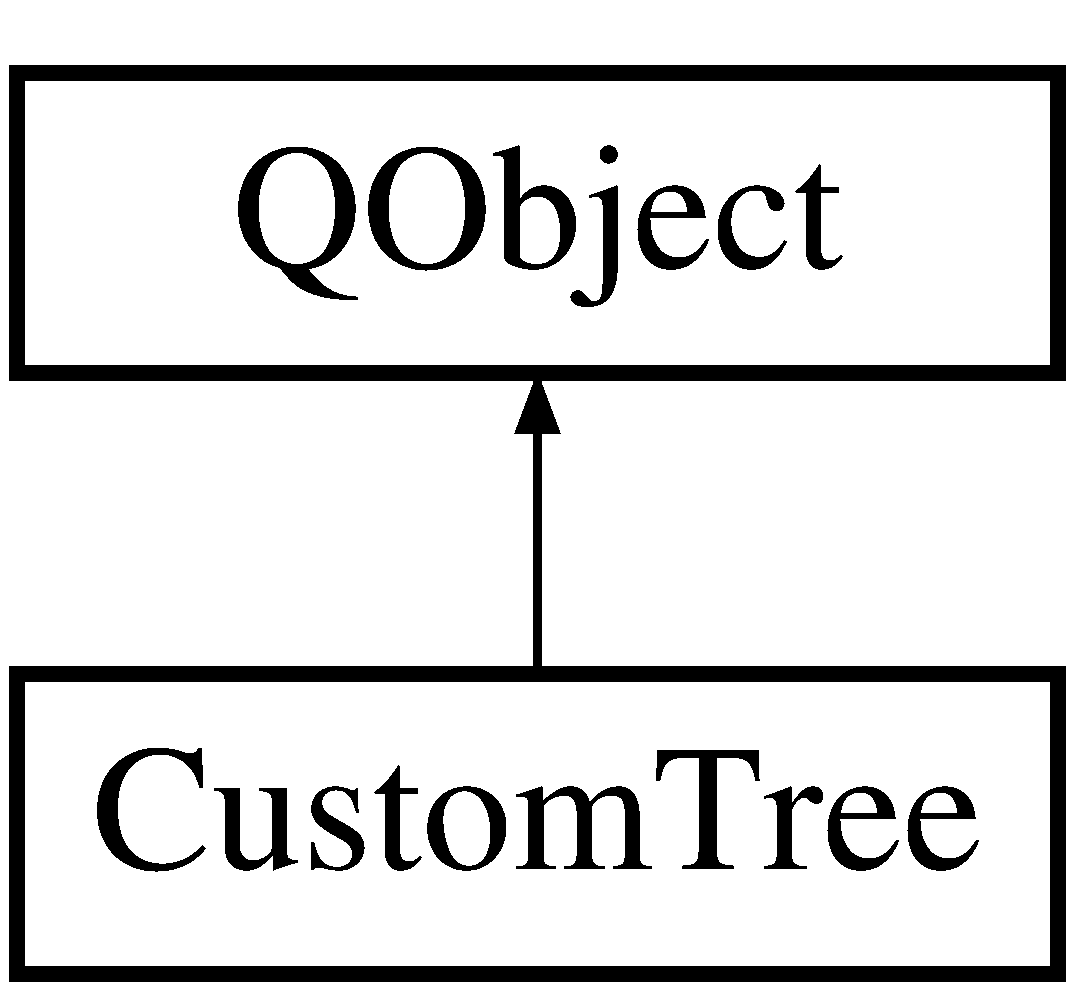
\includegraphics[height=2.000000cm]{class_custom_tree}
\end{center}
\end{figure}
\subsection*{Public Slots}
\begin{DoxyCompactItemize}
\item 
\mbox{\Hypertarget{class_custom_tree_adad1ea5f153ee963af8ec30725c56023}\label{class_custom_tree_adad1ea5f153ee963af8ec30725c56023}} 
void \hyperlink{class_custom_tree_adad1ea5f153ee963af8ec30725c56023}{check\+Selected} ()
\begin{DoxyCompactList}\small\item\em Метод который проверяет количество выделеных файлов в рабочей области. \end{DoxyCompactList}\item 
\mbox{\Hypertarget{class_custom_tree_a55beb6f033c52341c36a2a8dfc2a1f9f}\label{class_custom_tree_a55beb6f033c52341c36a2a8dfc2a1f9f}} 
void \hyperlink{class_custom_tree_a55beb6f033c52341c36a2a8dfc2a1f9f}{draw\+Path} ()
\begin{DoxyCompactList}\small\item\em отрисовка пути до выделенного файла в UI. \end{DoxyCompactList}\item 
\mbox{\Hypertarget{class_custom_tree_a74d1a0175ab32ba81ddb263b2e276196}\label{class_custom_tree_a74d1a0175ab32ba81ddb263b2e276196}} 
void \hyperlink{class_custom_tree_a74d1a0175ab32ba81ddb263b2e276196}{open\+Item} ()
\begin{DoxyCompactList}\small\item\em open\+Item -\/ Конструкция, открывающая файл по нажатию двойного щелчка. \end{DoxyCompactList}\item 
void \hyperlink{class_custom_tree_a183106efb54d0ce0d24da6bdb537002b}{pop\+Up} ()
\item 
void \hyperlink{class_custom_tree_a66a79068ff84c6e74290c9ba0709f770}{popup\+Copy} ()
\begin{DoxyCompactList}\small\item\em Метод, где все выделенные файлы загружаются в Q\+List$<$\+Q\+String$>$. Также используется и для вырезания, и для удаления, но немного иначе. \end{DoxyCompactList}\item 
\mbox{\Hypertarget{class_custom_tree_ae5f00ca23c452d55edee58e7699347c1}\label{class_custom_tree_ae5f00ca23c452d55edee58e7699347c1}} 
void {\bfseries popup\+Cut} ()
\item 
\mbox{\Hypertarget{class_custom_tree_ac209cddc61a0a469a8f7c658b4a043a4}\label{class_custom_tree_ac209cddc61a0a469a8f7c658b4a043a4}} 
void \hyperlink{class_custom_tree_ac209cddc61a0a469a8f7c658b4a043a4}{popup\+Paste} ()
\begin{DoxyCompactList}\small\item\em Метод вставки выделенных файлов/каталогов. \end{DoxyCompactList}\item 
\mbox{\Hypertarget{class_custom_tree_accdc09b7ceea8a35c7942fb9924dce1a}\label{class_custom_tree_accdc09b7ceea8a35c7942fb9924dce1a}} 
void \hyperlink{class_custom_tree_accdc09b7ceea8a35c7942fb9924dce1a}{popup\+Erase} ()
\begin{DoxyCompactList}\small\item\em метод удаления выделеных файлов/директорий \end{DoxyCompactList}\item 
\mbox{\Hypertarget{class_custom_tree_a8bbf60d9a3a0013f06e0c1f664c1232d}\label{class_custom_tree_a8bbf60d9a3a0013f06e0c1f664c1232d}} 
void {\bfseries popup\+Rename} ()
\item 
\mbox{\Hypertarget{class_custom_tree_ade7eaee5334057660fc809135a552ff5}\label{class_custom_tree_ade7eaee5334057660fc809135a552ff5}} 
void {\bfseries popup\+Prop} ()
\item 
\mbox{\Hypertarget{class_custom_tree_a3cf5d572ab9c17bb1d1de3bf5b3bff32}\label{class_custom_tree_a3cf5d572ab9c17bb1d1de3bf5b3bff32}} 
void {\bfseries popup\+Mkdir} ()
\item 
\mbox{\Hypertarget{class_custom_tree_ae5b4a2f7ebd76218da697b05f367231c}\label{class_custom_tree_ae5b4a2f7ebd76218da697b05f367231c}} 
void {\bfseries refresh\+Tree} ()
\item 
\mbox{\Hypertarget{class_custom_tree_adc8adaa0a30d1fc981a724cb0b8265df}\label{class_custom_tree_adc8adaa0a30d1fc981a724cb0b8265df}} 
void \hyperlink{class_custom_tree_adc8adaa0a30d1fc981a724cb0b8265df}{debug} ()
\begin{DoxyCompactList}\small\item\em этот метод не несет в себе никакого смысла, создан для отладки. \end{DoxyCompactList}\end{DoxyCompactItemize}
\subsection*{Public Member Functions}
\begin{DoxyCompactItemize}
\item 
\mbox{\Hypertarget{class_custom_tree_a8bdf32ee5de09eef817afec6e721a309}\label{class_custom_tree_a8bdf32ee5de09eef817afec6e721a309}} 
\hyperlink{class_custom_tree_a8bdf32ee5de09eef817afec6e721a309}{Custom\+Tree} (Q\+Object $\ast$parent=nullptr)
\begin{DoxyCompactList}\small\item\em Здесь налаживаются все связи между событиями. \end{DoxyCompactList}\item 
\mbox{\Hypertarget{class_custom_tree_ab276e0f77be6238627b0f12186407bc6}\label{class_custom_tree_ab276e0f77be6238627b0f12186407bc6}} 
void {\bfseries add\+Path} (Q\+Line\+Edit $\ast$Line\+Edit)
\item 
\mbox{\Hypertarget{class_custom_tree_acc5b99990df42d12c48bc67f8e099455}\label{class_custom_tree_acc5b99990df42d12c48bc67f8e099455}} 
void {\bfseries add\+Other\+Path} (Q\+Line\+Edit $\ast$Line\+Edit)
\item 
\mbox{\Hypertarget{class_custom_tree_a045dd1fa2368a162ac7dabb326f4f256}\label{class_custom_tree_a045dd1fa2368a162ac7dabb326f4f256}} 
void {\bfseries add\+File\+Name} (Q\+Line\+Edit $\ast$Line\+Edit)
\item 
\mbox{\Hypertarget{class_custom_tree_ad9a3782f13e222a141aeafade2edfc61}\label{class_custom_tree_ad9a3782f13e222a141aeafade2edfc61}} 
void {\bfseries add\+Tab} (Q\+Tab\+Widget $\ast$tab)
\item 
\mbox{\Hypertarget{class_custom_tree_af43b1fea3a6597175cd1c227c77e916e}\label{class_custom_tree_af43b1fea3a6597175cd1c227c77e916e}} 
void {\bfseries add\+Tree} (Q\+Tree\+View $\ast$tree)
\item 
\mbox{\Hypertarget{class_custom_tree_a48fe77a51f2ec17c6f6688b51c0a3a54}\label{class_custom_tree_a48fe77a51f2ec17c6f6688b51c0a3a54}} 
bool {\bfseries erase\+Dir} (Q\+Model\+Index index)
\item 
\mbox{\Hypertarget{class_custom_tree_a0de6a7896af48da2a1a7ee4e84851576}\label{class_custom_tree_a0de6a7896af48da2a1a7ee4e84851576}} 
void {\bfseries add\+Model} (Q\+Dir\+Model $\ast$model)
\item 
\mbox{\Hypertarget{class_custom_tree_a004e09ac9843c95093be3087fa7b4224}\label{class_custom_tree_a004e09ac9843c95093be3087fa7b4224}} 
void {\bfseries add\+Bool} (bool \&E\+M\+P\+TY)
\item 
\mbox{\Hypertarget{class_custom_tree_ae72ee91343f0b84f04289ff640350f07}\label{class_custom_tree_ae72ee91343f0b84f04289ff640350f07}} 
void {\bfseries add\+Cut} (bool \&C\+UT)
\item 
\mbox{\Hypertarget{class_custom_tree_a588b7b357c6efd6479fe2dddcb55adbb}\label{class_custom_tree_a588b7b357c6efd6479fe2dddcb55adbb}} 
void {\bfseries add\+Clipboard} (Q\+Model\+Index \&SI)
\item 
\mbox{\Hypertarget{class_custom_tree_afe4e3fa1b690292c90273b0d3452c70f}\label{class_custom_tree_afe4e3fa1b690292c90273b0d3452c70f}} 
void {\bfseries add\+Count} (qint32 \&SC)
\item 
\mbox{\Hypertarget{class_custom_tree_ad885c6ead133dc48af4ec300f5a38e23}\label{class_custom_tree_ad885c6ead133dc48af4ec300f5a38e23}} 
void {\bfseries add\+Vec} (Q\+List$<$ Q\+String $>$ \&L)
\item 
void \hyperlink{class_custom_tree_a3687c6feff0539eec56582ff95239589}{event\+Handle} (Q\+Key\+Event $\ast$event)
\item 
bool \hyperlink{class_custom_tree_a373ba76bdc9886cd2e997d5af84a0cba}{scan\+Dir} (std\+::wstring old\+File, std\+::wstring new\+File, boost\+::system\+::error\+\_\+code error\+\_\+code)
\end{DoxyCompactItemize}
\subsection*{Static Public Attributes}
\begin{DoxyCompactItemize}
\item 
\mbox{\Hypertarget{class_custom_tree_a0db9d3bfff8ac0d3a0509959210621b2}\label{class_custom_tree_a0db9d3bfff8ac0d3a0509959210621b2}} 
static const char {\bfseries slash} = \textquotesingle{}/\textquotesingle{}
\item 
\mbox{\Hypertarget{class_custom_tree_a29b0f6e5a661df1478b820c96baabe09}\label{class_custom_tree_a29b0f6e5a661df1478b820c96baabe09}} 
static const char {\bfseries non\+Slash} = \textquotesingle{}\textbackslash{}\textbackslash{}\textquotesingle{}
\end{DoxyCompactItemize}


\subsection{Detailed Description}
Класс посредник 

В этот класс в самом начале закидываются все необходимые элементы управления, переменные, объекты, чтобы далее с ними было проще обращаться из одног места. 

\subsection{Member Function Documentation}
\mbox{\Hypertarget{class_custom_tree_a3687c6feff0539eec56582ff95239589}\label{class_custom_tree_a3687c6feff0539eec56582ff95239589}} 
\index{Custom\+Tree@{Custom\+Tree}!event\+Handle@{event\+Handle}}
\index{event\+Handle@{event\+Handle}!Custom\+Tree@{Custom\+Tree}}
\subsubsection{\texorpdfstring{event\+Handle()}{eventHandle()}}
{\footnotesize\ttfamily void Custom\+Tree\+::event\+Handle (\begin{DoxyParamCaption}\item[{Q\+Key\+Event $\ast$}]{event }\end{DoxyParamCaption})}

Пока не используется T\+O\+DO -\/ Обработчик горячих клавиш. \mbox{\Hypertarget{class_custom_tree_a183106efb54d0ce0d24da6bdb537002b}\label{class_custom_tree_a183106efb54d0ce0d24da6bdb537002b}} 
\index{Custom\+Tree@{Custom\+Tree}!pop\+Up@{pop\+Up}}
\index{pop\+Up@{pop\+Up}!Custom\+Tree@{Custom\+Tree}}
\subsubsection{\texorpdfstring{pop\+Up}{popUp}}
{\footnotesize\ttfamily void Custom\+Tree\+::pop\+Up (\begin{DoxyParamCaption}{ }\end{DoxyParamCaption})\hspace{0.3cm}{\ttfamily [slot]}}

Метод происходит, когда выпадает контекствое меню. Здесь включаются и выключаются необходимые кнопки. \mbox{\Hypertarget{class_custom_tree_a66a79068ff84c6e74290c9ba0709f770}\label{class_custom_tree_a66a79068ff84c6e74290c9ba0709f770}} 
\index{Custom\+Tree@{Custom\+Tree}!popup\+Copy@{popup\+Copy}}
\index{popup\+Copy@{popup\+Copy}!Custom\+Tree@{Custom\+Tree}}
\subsubsection{\texorpdfstring{popup\+Copy}{popupCopy}}
{\footnotesize\ttfamily void Custom\+Tree\+::popup\+Copy (\begin{DoxyParamCaption}{ }\end{DoxyParamCaption})\hspace{0.3cm}{\ttfamily [slot]}}



Метод, где все выделенные файлы загружаются в Q\+List$<$\+Q\+String$>$. Также используется и для вырезания, и для удаления, но немного иначе. 

Если коротко, то здесь программа запоминает все выделенные файлы. \mbox{\Hypertarget{class_custom_tree_a373ba76bdc9886cd2e997d5af84a0cba}\label{class_custom_tree_a373ba76bdc9886cd2e997d5af84a0cba}} 
\index{Custom\+Tree@{Custom\+Tree}!scan\+Dir@{scan\+Dir}}
\index{scan\+Dir@{scan\+Dir}!Custom\+Tree@{Custom\+Tree}}
\subsubsection{\texorpdfstring{scan\+Dir()}{scanDir()}}
{\footnotesize\ttfamily bool Custom\+Tree\+::scan\+Dir (\begin{DoxyParamCaption}\item[{std\+::wstring}]{old\+File,  }\item[{std\+::wstring}]{new\+File,  }\item[{boost\+::system\+::error\+\_\+code}]{error\+\_\+code }\end{DoxyParamCaption})}

This function provides recursively copy the folder and files. Эта функция позволяет рекурсивно делать копии папок и файлов. 

The documentation for this class was generated from the following files\+:\begin{DoxyCompactItemize}
\item 
customtree.\+h\item 
customtree.\+cpp\end{DoxyCompactItemize}

\hypertarget{class_main_window}{}\section{Main\+Window Class Reference}
\label{class_main_window}\index{Main\+Window@{Main\+Window}}


\hyperlink{class_main_window}{Main\+Window} -\/ Главный фрейм, который создаётся автоматически.  




{\ttfamily \#include $<$mainwindow.\+h$>$}

Inheritance diagram for Main\+Window\+:\begin{figure}[H]
\begin{center}
\leavevmode
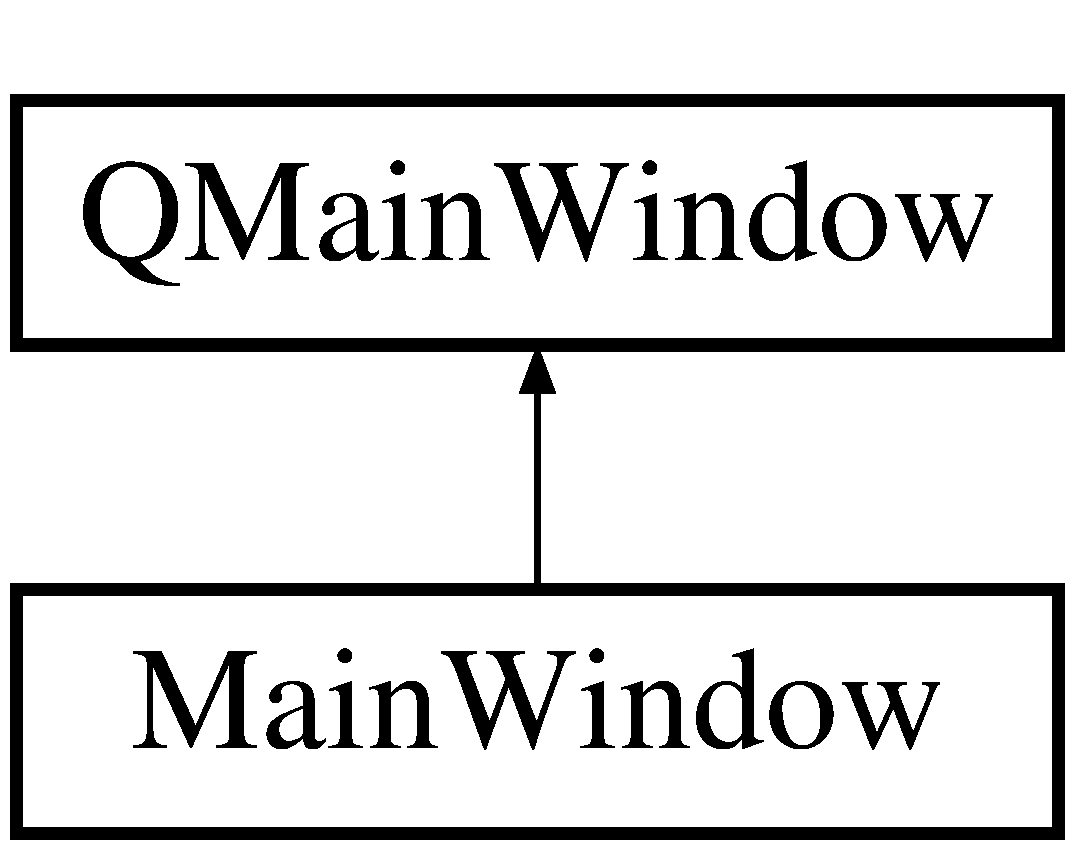
\includegraphics[height=2.000000cm]{class_main_window}
\end{center}
\end{figure}
\subsection*{Public Slots}
\begin{DoxyCompactItemize}
\item 
\mbox{\Hypertarget{class_main_window_aaab29f305f38d7e4cca212c97a442536}\label{class_main_window_aaab29f305f38d7e4cca212c97a442536}} 
bool {\bfseries event} (Q\+Event $\ast$event)
\end{DoxyCompactItemize}
\subsection*{Public Member Functions}
\begin{DoxyCompactItemize}
\item 
\mbox{\Hypertarget{class_main_window_a8b244be8b7b7db1b08de2a2acb9409db}\label{class_main_window_a8b244be8b7b7db1b08de2a2acb9409db}} 
{\bfseries Main\+Window} (Q\+Widget $\ast$parent=0)
\end{DoxyCompactItemize}
\subsection*{Public Attributes}
\begin{DoxyCompactItemize}
\item 
\mbox{\Hypertarget{class_main_window_aea75eabd1a2a44e904eebfee4bede93d}\label{class_main_window_aea75eabd1a2a44e904eebfee4bede93d}} 
bool \hyperlink{class_main_window_aea75eabd1a2a44e904eebfee4bede93d}{empty} = true
\begin{DoxyCompactList}\small\item\em Clipboard на самом деле это не буфер обмена, но нечто похожее. Эдакий внутре-\/программный буфер. Можно было воспользоваться библиотекой Q\+Clipboard, но я посчитал это слишком для моего маленького проекта. \end{DoxyCompactList}\item 
\mbox{\Hypertarget{class_main_window_a16f874cb7a61706ee8ca30b21578f9ec}\label{class_main_window_a16f874cb7a61706ee8ca30b21578f9ec}} 
bool {\bfseries cutted} = false
\item 
\mbox{\Hypertarget{class_main_window_a4e9ddafd764926ca67ea77e564f15677}\label{class_main_window_a4e9ddafd764926ca67ea77e564f15677}} 
int {\bfseries selected\+Count}
\item 
\mbox{\Hypertarget{class_main_window_a67f685d445845eb32195a6392400d082}\label{class_main_window_a67f685d445845eb32195a6392400d082}} 
Q\+Model\+Index {\bfseries selected\+Index}
\end{DoxyCompactItemize}


\subsection{Detailed Description}
\hyperlink{class_main_window}{Main\+Window} -\/ Главный фрейм, который создаётся автоматически. 

The documentation for this class was generated from the following files\+:\begin{DoxyCompactItemize}
\item 
mainwindow.\+h\item 
mainwindow.\+cpp\end{DoxyCompactItemize}

\hypertarget{class_prop}{}\section{Prop Class Reference}
\label{class_prop}\index{Prop@{Prop}}


\hyperlink{class_prop}{Prop} (Properties) -\/ Класс отображающий свойство файла. Если в кратце, то просто очень сырой и не нужный.  




{\ttfamily \#include $<$prop.\+h$>$}

Inheritance diagram for Prop\+:\begin{figure}[H]
\begin{center}
\leavevmode
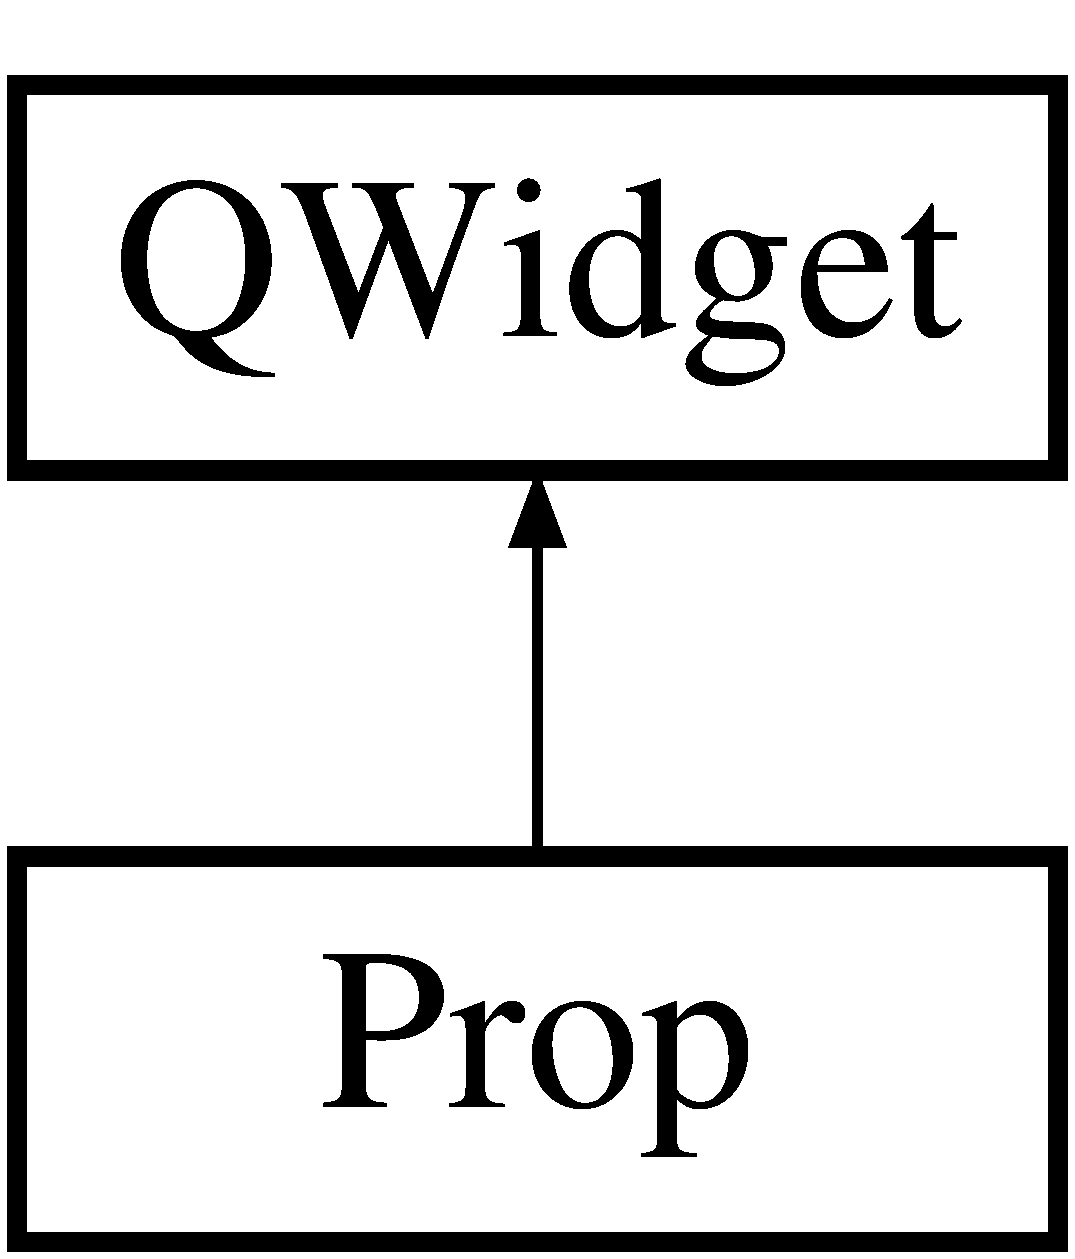
\includegraphics[height=2.000000cm]{class_prop}
\end{center}
\end{figure}
\subsection*{Public Member Functions}
\begin{DoxyCompactItemize}
\item 
\mbox{\Hypertarget{class_prop_a14a5bfb4b751a2d65516d4d7724f4cae}\label{class_prop_a14a5bfb4b751a2d65516d4d7724f4cae}} 
{\bfseries Prop} (Q\+String name=\char`\"{}Title\char`\"{}, Q\+Widget $\ast$parent=0)
\item 
\mbox{\Hypertarget{class_prop_a126f5332ae79e0b924f17c81e8529bcc}\label{class_prop_a126f5332ae79e0b924f17c81e8529bcc}} 
void {\bfseries set\+Name\+Edit} (Q\+String name)
\item 
\mbox{\Hypertarget{class_prop_af4b5a88ba0af1f317768e5695a3454d2}\label{class_prop_af4b5a88ba0af1f317768e5695a3454d2}} 
void {\bfseries set\+Size\+Edit} (Q\+String name)
\item 
\mbox{\Hypertarget{class_prop_a24b678764b43b8fd932631aec6e80011}\label{class_prop_a24b678764b43b8fd932631aec6e80011}} 
void {\bfseries set\+Path\+Edit} (Q\+String name)
\end{DoxyCompactItemize}


\subsection{Detailed Description}
\hyperlink{class_prop}{Prop} (Properties) -\/ Класс отображающий свойство файла. Если в кратце, то просто очень сырой и не нужный. 

The documentation for this class was generated from the following files\+:\begin{DoxyCompactItemize}
\item 
prop.\+h\item 
prop.\+cpp\end{DoxyCompactItemize}

%--- End generated contents ---

% Index
\backmatter
\newpage
\phantomsection
\clearemptydoublepage
\addcontentsline{toc}{chapter}{Index}
\printindex

\end{document}
